\documentclass[12pt, twoside]{article}
\usepackage[letterpaper, margin=1in, head=30pt, headsep=0.1in]{geometry}
\usepackage[english]{babel}
\usepackage[utf8]{inputenc}
\usepackage{amsmath}
\usepackage{amsfonts}
\usepackage{amssymb}
\usepackage{tikz}
%\usetikzlibrary{quotes, angles}

\usepackage{graphicx}
\usepackage{enumitem}
\usepackage{multicol}

\newif\ifmeta
\metatrue %print standards and topics tags

\title{Regents Geometry}
\author{Chris Huson}
\date{October 2021}

\usepackage{fancyhdr}
\pagestyle{fancy}
\fancyhf{}
\renewcommand{\headrulewidth}{0pt} % disable the underline of the header
\raggedbottom


\fancyhead[LE]{\thepage}
\fancyhead[RO]{\thepage \\ Name: \hspace{4cm} \,\\}
\fancyhead[LO]{BECA / Dr. Huson / Geometry 04 Analytic Geometry}

\begin{document}

\subsubsection*{4.2 Distance Formula}
\begin{enumerate}
\item Do Now: Use a centimeter ruler to measure the triangle side lengths.
\begin{flushright}
  \begin{tikzpicture}[scale=1]
    \node at (4,3)[above left]{$c$};
    \node at (8,3)[right]{6 cm};
    \node at (4,0)[below]{8 cm};
    \draw [thick] (0, 0)--(8, 0)--(8, 6)--cycle;
    \draw [dashed] (8,0)++(-0.4,0)-- ++(0,0.4)-- +(0.4,0);
  \end{tikzpicture}
\end{flushright}

  
Note: The formula for distance is $\displaystyle d=\sqrt{(x_2-x_1)^2+(y_2-y_1)^2}$

\item Graph and label $\triangle ABC$. Calculate the lengths of its sides. $A(1,2)$, $B(9,8)$, $C(9,2)$.
    \begin{enumerate}
      \begin{multicols}{2}
      \item   $AC=$ \vspace{1.cm}
      \item   $BC=$ \vspace{1.cm}
      \item   $AB=$ \vspace{3cm}
        \begin{center}
          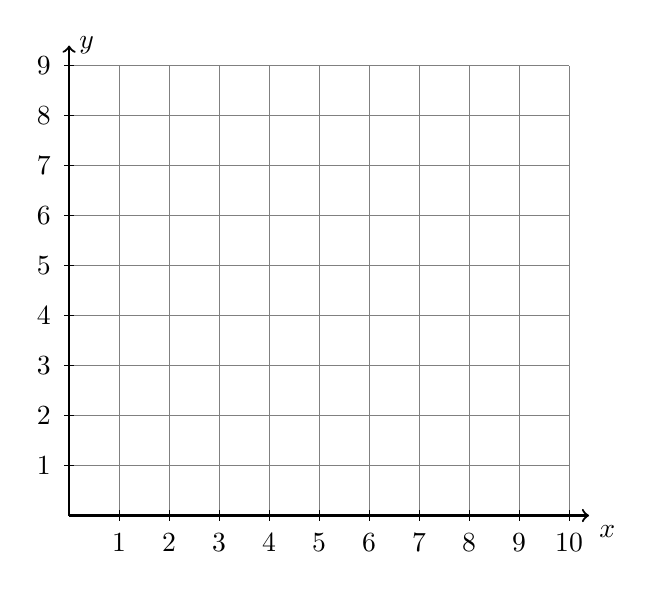
\begin{tikzpicture}[scale=.635]
            \draw [help lines] (0,0) grid (10,9);
            \draw [thick, ->] (0,0) -- (10.4,0) node [below right] {$x$};
            \draw [thick, ->] (0,0)--(0,9.4) node [right] {$y$};
            \foreach \x in {1,...,10}
            \draw[shift={(\x,0)}] (0pt,-3pt)--(0pt,3pt) node[below=5pt] {$\x$};
            \foreach \y in {1,...,9}
            \draw[shift={(0,\y)}] (-3pt,0pt)--(3pt,0pt) node[left=5pt] {$\y$};
          \end{tikzpicture}
          \end{center}
      \end{multicols}
    \end{enumerate}
  
\item What is the length of $\overline{CD}$ if $C(3,-1)$ and $D(-2,11)$?

\newpage
\item Graph and label $\triangle ABC$. Calculate the lengths of its sides. $A(0,0)$, $B(12,5)$, $C(12,0)$.
\begin{flushleft}
  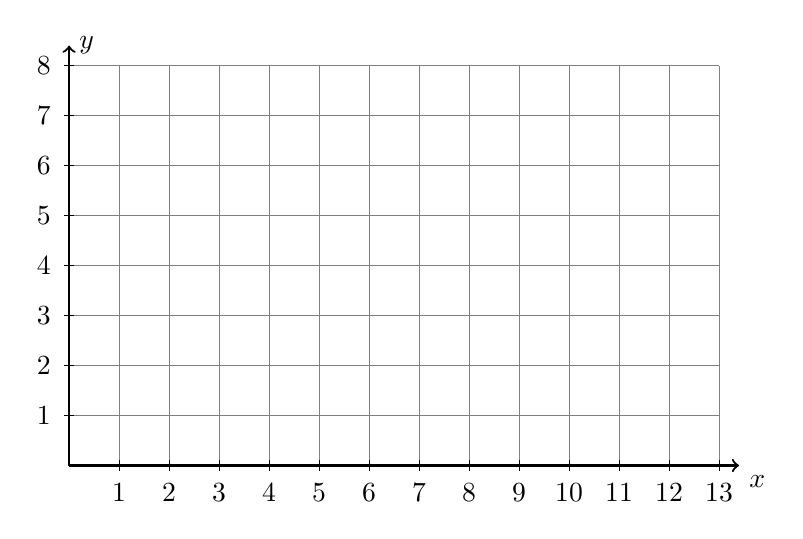
\begin{tikzpicture}[scale=.635]
    \draw [help lines] (0,0) grid (13,8);
    \draw [thick, ->] (0,0) -- (13.4,0) node [below right] {$x$};
    \draw [thick, ->] (0,0)--(0,8.4) node [right] {$y$};
    \foreach \x in {1,...,13}
    \draw[shift={(\x,0)}] (0pt,-3pt)--(0pt,3pt) node[below=5pt] {$\x$};
    \foreach \y in {1,...,8}
    \draw[shift={(0,\y)}] (-3pt,0pt)--(3pt,0pt) node[left=5pt] {$\y$};
  \end{tikzpicture}
\end{flushleft}

\item On the graph below, draw $\overline{EF}$, with $E(3,5)$ and $F(9,1)$, labeling the end points. Determine and state the coordinates of the midpoint $M$ of $\overline{EF}$ and mark and label it on the graph.
\begin{flushright}
  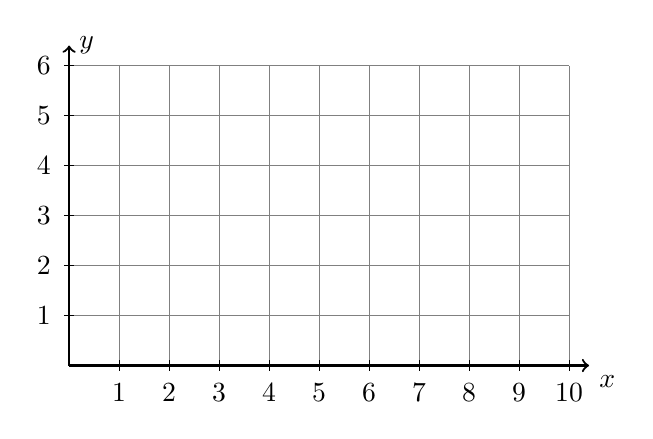
\begin{tikzpicture}[scale=.635]
    \draw [help lines] (0,0) grid (10,6);
    \draw [thick, ->] (0,0) -- (10.4,0) node [below right] {$x$};
    \draw [thick, ->] (0,0)--(0,6.4) node [right] {$y$};
    \foreach \x in {1,...,10}
    \draw[shift={(\x,0)}] (0pt,-3pt)--(0pt,3pt) node[below=5pt] {$\x$};
    \foreach \y in {1,...,6}
    \draw[shift={(0,\y)}] (-3pt,0pt)--(3pt,0pt) node[left=5pt] {$\y$};
  \end{tikzpicture}
\end{flushright}


\item Spicy: In  $\triangle ABC$ shown below, $m\angle A=(10x)^\circ$, $m\angle B=(16x-5)^\circ$, and $m\angle C=(2x+3)^\circ$. \\[0.25cm] 
  Find $m\angle A$. (show the check for full credit)
  \begin{flushright}
      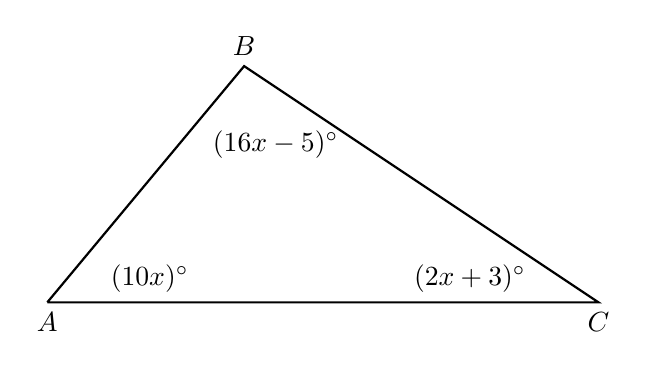
\begin{tikzpicture}
        \draw [thick]
          (2,0)node[below]{$A$}--
          (9,0)node[below]{$C$}--
          (4.5,3)node[above]{$B$} --(2,0);
          \node at (3.3,0)[above]{$(10x)^\circ$};
          \node at (8.2,0)[above left]{$(2x+3)^\circ$};
          \node at (4.9,2.3)[below]{$(16x-5)^\circ$};
      \end{tikzpicture}
    \end{flushright}

\end{enumerate}
\end{document}
